% PolluTrace -- AI4015 Agentic AI, Phase 2 paper (IEEEtran conference, 8-10 pages incl. references).
% BUILD: Overleaf (upload this folder as a ZIP) or `latexmk -pdf main.tex`.
% RULES (course): the text must be written by us, in our own words; no AI-generated writing.
%   Every number must come from results/ in the repo: tables in tables/*.tex are generated by
%   `python paper/make_tables.py`; quote numbers from those tables or results/phase2_tables.md only.
%   Every entry in refs.bib must be cited; run `python paper/check_refs.py`.
% The comments under each section list what the course requires there and which of our
% results/figures belong to it. They are notes for us, not text for the paper. Delete them
% before submission.
\documentclass[conference]{IEEEtran}
\usepackage[T1]{fontenc}
\usepackage{cite}
\usepackage{amsmath,amssymb}
\usepackage{graphicx}
\usepackage{booktabs}
\usepackage{multirow}
\usepackage{xcolor}
\usepackage{tikz}
\usetikzlibrary{positioning,arrows.meta,fit,calc}
\usepackage{url}
\usepackage[hidelinks]{hyperref}
\def\BibTeX{{\rm B\kern-.05em{\sc i\kern-.025em b}\kern-.08em T\kern-.1667em\lower.7ex\hbox{E}\kern-.125em X}}
\newcommand{\todo}[1]{\textcolor{red}{[TODO: #1]}}

\begin{document}

\title{PolluTrace: Execution-Grounded Multi-Agent Localization and Repair of Order-Dependent Flaky Tests\\
\large Project Code: SELF}

\author{
\IEEEauthorblockN{Zoya Ahmad (Group Head)}
\IEEEauthorblockA{Roll No. 23I-0805\\
Department of Computer Science\\
FAST-NUCES, Islamabad, Pakistan\\
\todo{email}}
\and
\IEEEauthorblockN{Zarpash Nasim}
\IEEEauthorblockA{Roll No. 23I-0027\\
Department of Computer Science\\
FAST-NUCES, Islamabad, Pakistan\\
\todo{email}}
\and
\IEEEauthorblockN{Supervisor: Muhammad Sajjad}
\IEEEauthorblockA{Department of Computer Science\\
FAST-NUCES, Islamabad, Pakistan}
}

\maketitle

% ===================================================================== 1
\begin{abstract}
% 150-250 words. Problem; approach; main quantitative results (fix rate, false-fix rate,
% localization cost from tables/main.tex and tables/gap.tex); contribution.
% Write LAST, after the results are final.
\todo{abstract}
\end{abstract}

\begin{IEEEkeywords}
flaky tests, order-dependent tests, LLM agents, automated program repair, test pollution
\end{IEEEkeywords}

% ===================================================================== 2
\section{Introduction}
\label{sec:intro}
% Owner: Zoya.
% - Motivation: flaky tests, OD tests as a major class [luo2014empirical, parry2021survey,
%   zhang2014independence]; cost in CI.
% - Current tools: iDFlakies/iFixFlakies [lam2019idflakies, shi2019ifixflakies], ODRepair
%   [li2022odrepair], LLM-based repair [chen2024flakydoctor, fatima2024flakyfix, li2025flakyguard],
%   base paper NIODebugger [ke2025niodebugger].
% - The three gaps from Phase 1 (G1 blind polluter search, G2 repair without state evidence,
%   G3 acceptance after a single passing run).
% - Research questions RQ1-RQ3 (one per gap) + RQ4 (cost/reliability).
% - Contributions list (system, harness/benchmark protocol, empirical study, open repository).
\todo{introduction}

% ===================================================================== 3
\section{Related Work}
\label{sec:related}
% Owner: Zoya. Synthesis of the Phase 1 review, grouped by theme, NOT one paragraph per paper.
% (a) Detecting and localizing OD tests: lam2019idflakies, gyori2015poldet, bell2015electrictest,
%     zhang2014independence, li2022evolution, li2023systematic, rahman2025rankf, iqbal2025reruns,
%     hashemi2025jsod, hashemi2026jstod, wang2022ipflakies, levin2025takuan.
% (b) Repairing flaky tests: shi2019ifixflakies, li2022odrepair, chen2024flakydoctor,
%     fatima2024flakyfix, li2025flakyguard, ke2025niodebugger, wei2022nio.
% (c) Flakiness studies: luo2014empirical, parry2021survey, parry2025systemic, parry2026flimsiness,
%     berndt2026llmflaky, berndt2026saphana.
% (d) LLM agents for SE and their evaluation: yao2023react, shinn2023reflexion, bouzenia2025repairagent,
%     xia2025agentless, jimenez2024swebench, yang2024sweagent, wang2026swebench.
% End with how PolluTrace differs from the base paper (OD pairs, execution-confirmed
% localization, state diff, strict validation).
\todo{related work}

% ===================================================================== 4
\section{Problem Formulation}
\label{sec:problem}
% Owner: Zoya.
% - Definitions: test suite T, order o, victim v, polluter p (v passes alone, fails after p in one JVM).
% - Task input: failing order o_f = (t_1..t_k, v) and failure trace; NOT the polluter list.
% - Output: a patch to a test class such that v passes in o_f, after every known polluter,
%   in N randomized orders, without weakening assertions (integrity).
% - Hypotheses H1-H3 (one per gap), stated so the experiments in Sec. VIII can confirm/reject them.
\todo{problem formulation}

% ===================================================================== 5
\section{Proposed System}
\label{sec:method}
% Owner: Zarpash. Architecture (Fig.~\ref{fig:arch}); agents, tools, state, and which component
% addresses which gap: localizer (G1), state diff (G2), repair, validator (G3), supervisor
% (budgets, feedback, backtracking). Code: pollutrace/agents/*, pollutrace/supervisor.py.
\todo{methodology}

\begin{figure*}[t]
  \centering
  % Architecture of PolluTrace (TikZ). Used by main.tex as Fig. 1.
\resizebox{\textwidth}{!}{%
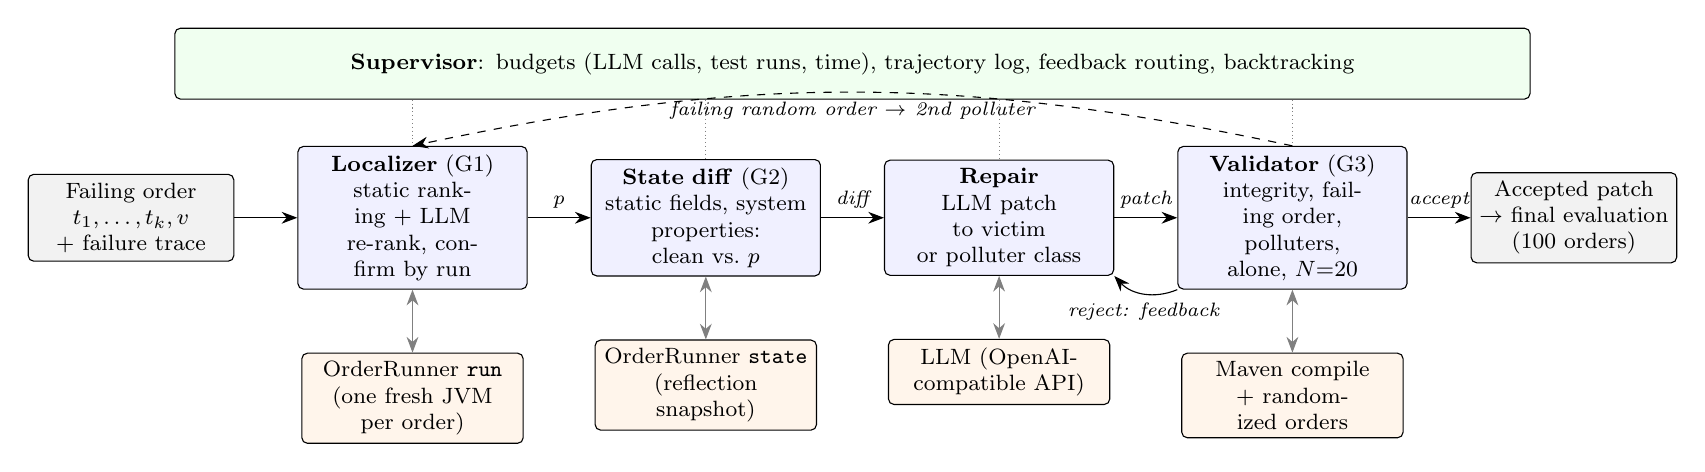
\begin{tikzpicture}[
  font=\footnotesize, >={Stealth[length=2mm]},
  box/.style={draw, rounded corners=2pt, align=center, minimum height=9mm, inner sep=3pt, fill=white},
  agent/.style={box, fill=blue!6, text width=27mm},
  io/.style={box, fill=gray!10, text width=24mm},
  tool/.style={box, fill=orange!8, text width=26mm, minimum height=7mm},
  lab/.style={font=\scriptsize\itshape, align=center}]
  \node[io] (in) {Failing order\\$t_1,\dots,t_k,v$\\+ failure trace};
  \node[agent, right=8mm of in] (loc) {\textbf{Localizer} (G1)\\static ranking + LLM\\re-rank, confirm by run};
  \node[agent, right=8mm of loc] (sd) {\textbf{State diff} (G2)\\static fields, system\\properties: clean vs.\ $p$};
  \node[agent, right=8mm of sd] (rep) {\textbf{Repair}\\LLM patch to victim\\or polluter class};
  \node[agent, right=8mm of rep] (val) {\textbf{Validator} (G3)\\integrity, failing order,\\polluters, alone, $N{=}20$};
  \node[io, right=8mm of val] (out) {Accepted patch\\$\rightarrow$ final evaluation\\(100 orders)};
  \node[box, fill=green!6, text width=170mm, above=15mm of $(loc)!0.5!(val)$] (sup)
       {\textbf{Supervisor}: budgets (LLM calls, test runs, time), trajectory log, feedback routing, backtracking};
  \node[tool, below=8mm of loc] (run) {OrderRunner \texttt{run}\\(one fresh JVM per order)};
  \node[tool, below=8mm of sd] (state) {OrderRunner \texttt{state}\\(reflection snapshot)};
  \node[tool, below=8mm of rep] (llm) {LLM (OpenAI-\\compatible API)};
  \node[tool, below=8mm of val] (mvn) {Maven compile\\+ randomized orders};
  \draw[->] (in) -- (loc);
  \draw[->] (loc) -- node[above, lab]{$p$} (sd);
  \draw[->] (sd) -- node[above, lab]{diff} (rep);
  \draw[->] (rep) -- node[above, lab]{patch} (val);
  \draw[->] (val) -- node[above, lab]{accept} (out);
  \draw[->] (val.south west) to[bend left=35] node[below, lab, pos=0.5]{reject: feedback} (rep.south east);
  \draw[->, dashed] (val.north) to[bend right=12] node[below, lab, pos=0.5]{failing random order $\rightarrow$ 2nd polluter} (loc.north);
  \foreach \a/\t in {loc/run, sd/state, rep/llm, val/mvn} \draw[<->, gray] (\a) -- (\t);
  \foreach \a in {loc, sd, rep, val} \draw[gray, densely dotted] (sup.south -| \a.north) -- (\a.north);
\end{tikzpicture}}

  \caption{PolluTrace architecture. \todo{caption in our words}}
  \label{fig:arch}
\end{figure*}

% ===================================================================== 6
\section{Experimental Setup}
\label{sec:setup}
% Owner: Zarpash.
% - Dataset: IDoFT odr-tests (135 victims); reproduction 90/135 (Phase 1); dev set 15; test subset
%   (rule in scripts/make_subset.py; say which projects were dropped and why).
% - Fixed failing orders (harness.failing_order), toolchains (JDK 8/11/17), hardware.
% - Systems: B1, B2 (iFixFlakies), B4 (NIODebugger-style, reproduced by us), PolluTrace, A1-A3.
% - Model name/version, temperature 0.2, seeds, budgets (pollutrace/config.py), 3 runs.
% - No tuning on the test subset.
\todo{experimental setup}

% ===================================================================== 7
\section{Evaluation Methodology}
\label{sec:evalmethod}
% Owner: Zarpash. Metrics and how they are computed (eval/stats.py): fix rate, precision,
% false-fix rate (final 100 randomized orders), localization runs/executions, tokens, time.
% How the base-paper comparison is made (same harness, same victims, reproduced by us).
% Statistics: mean +- std over 3 runs; paired sign test.
\todo{evaluation methodology}

% ===================================================================== 8
\section{Results}
\label{sec:results}
% Organized by gap. Zoya: G1 and G3 subsections. Zarpash: G2 subsection.
\subsection{Overall comparison}
\begin{table*}[t]
\centering
\caption{Repair results on the test subset.}\label{tab:main}
\textit{results not yet generated: run python paper/make\_tables.py}
\end{table*}

\todo{discussion of Table~\ref{tab:main}}

\subsection{G1: Polluter localization}
\begin{table*}[t]
\centering
\footnotesize
\caption{E4-G1: cost of finding the polluter in the failing order (same orders and run budget).}
\label{tab:g1}
\begin{tabular}{lrrrrr}
\toprule
\textbf{Strategy} & \textbf{Trials} & \textbf{Known polluter found} & \textbf{Runs (mean)} & \textbf{Runs (median)} & \textbf{Test executions} \\
\midrule
Ranked + LLM (PolluTrace) & 12 & 92\% & 2.1 & 1 & 5 \\
Ranked, static only & 12 & 92\% & 1.8 & 2 & 4 \\
One-by-one (iDFlakies-style) & 12 & 92\% & 20.0 & 20 & 40 \\
Delta debugging (iFixFlakies-style) & 12 & 100\% & 9.2 & 8 & 60 \\
Random order & 12 & 92\% & 11.4 & 10 & 23 \\
\bottomrule
\end{tabular}
\end{table*}

\todo{G1 results (Zoya)}

\subsection{G2: State evidence for repair}
\begin{table}[t]
\centering
\footnotesize
\caption{E4-G2: state diff of the confirmed polluter, and its effect on repair.}
\label{tab:g2}
\begin{tabular}{lr}
\toprule
\textbf{Measure} & \textbf{Value} \\
\midrule
Victims with a state diff & 15 / 15 \\
Diff shows a changed field or property & 12 / 15 \\
Changed field in state the victim uses & 9 / 15 \\
Fields snapshotted per victim (median) & 82 \\
Fix rate with diff & 58.3\% \\
Fix rate without diff & 58.3\% \\
\bottomrule
\end{tabular}
\end{table}

\todo{G2 results (Zarpash)}

\subsection{G3: Validation}
\begin{table}[t]
\centering
\caption{E4-G3: seeded bad patches.}\label{tab:g3}
\textit{results not yet generated: run python paper/make\_tables.py}
\end{table}

\todo{G3 results (Zoya)}

\subsection{Gap-resolution summary}
\begin{table*}[t]
\centering
\caption{Gap-resolution table.}\label{tab:gap}
\textit{results not yet generated: run python paper/make\_tables.py}
\end{table*}

% Fill the "Addressed?" column ourselves (Fully/Partially/Not) from the evidence.

% ===================================================================== 9
\section{Ablation and Comparative Analysis}
\label{sec:ablation}
% Owner: Zarpash. A1-A3 vs full (tables/main.tex rows, paired tests), cost trade-offs
% (tables/efficiency.tex).
\begin{table*}[t]
\centering
\footnotesize
\caption{E6: cost per victim and reliability across runs (mean $\pm$ std over runs).}
\label{tab:eff}
\begin{tabular}{lrrrrrrr}
\toprule
\textbf{System} & \textbf{LLM calls} & \textbf{Prompt tok.} & \textbf{Compl. tok.} & \textbf{USD} & \textbf{Test runs} & \textbf{Agent s} & \textbf{Same outcome} \\
\midrule
B1 single LLM call & 1.0 & 6113.3 & 5273.2 & 0.0150 & 0.0 & 10.3 & 12/12 \\
B4 NIODebugger-style (base paper, ours) & 1.8 & 17867.8 & 13449.4 & 0.0390 & 10.3 & 65.9 & 12/12 \\
PolluTrace (full) & 3.3 & 25393.9 & 17829.6 & 0.0522 & 18.3 & 100.9 & 12/12 \\
A1 without localizer (G1) & 2.7 & 23191.2 & 18079.7 & 0.0522 & 11.6 & 70.1 & 12/12 \\
A2 without state diff (G2) & 3.2 & 24454.4 & 18225.3 & 0.0529 & 16.2 & 71.0 & 12/12 \\
A3 weak validator (G3) & 3.2 & 24669.4 & 17535.6 & 0.0512 & 5.6 & 58.1 & 12/12 \\
\bottomrule
\end{tabular}
\end{table*}

\todo{ablation and efficiency}

% ===================================================================== 10
\section{Failure Analysis}
\label{sec:failures}
% Owner: Zoya. Categories and counts (tables/failures.tex from results/failure_analysis.md),
% likely cause + future fix per major category, 2 success + 2 failure trajectories
% (condensed in results/failure_analysis.md).
\begin{table*}[t]
\centering
\caption{Failure categories.}\label{tab:fail}
\textit{results not yet generated: run python paper/make\_tables.py}
\end{table*}

\todo{failure analysis}

% ===================================================================== 11
\section{Limitations and Threats to Validity}
\label{sec:threats}
% Owner: Zarpash. Internal (heuristic integrity check, single LLM, fixed failing order),
% external (Java/Maven only, IDoFT subset, dropped slow projects, 45 victims not reproducible),
% construct (randomized-order validation can still miss failures; B4 is a re-implementation).
\todo{limitations}

% ===================================================================== 12
\section{Conclusion}
\label{sec:conclusion}
% Both. Main findings per RQ; future work tied to the failure categories.
\todo{conclusion}

% ===================================================================== 13
\bibliographystyle{IEEEtran}
\bibliography{refs}

\end{document}
